%-------------------------------------------------------------------------------------------
% Vorlage erstellt von sli92
% Latex für Einsteiger: http://latex.mschroeder.net/#textformatierung
% Formeln in Latex: http://www.hosi.de/latex/mathe.htm
%-------------------------------------------------------------------------------------------
%PRÄAMBEL
%-------------------------------------------------------------------------------------------

\documentclass[a4paper,14pt,headsepline]{scrartcl}

\usepackage[ngerman]{babel}
\usepackage[utf8]{inputenc}
\usepackage{fancyheadings}
\usepackage{graphicx}
\usepackage{eurosym}

\usepackage{hyperref}

\usepackage{tabularx}
\newcolumntype{L}[1]{>{\raggedright\arraybackslash}p{#1}} % linksbündig mit Breitenangabe
\newcolumntype{C}[1]{>{\centering\arraybackslash}p{#1}} % zentriert mit Breitenangabe
\newcolumntype{R}[1]{>{\raggedleft\arraybackslash}p{#1}} % rechtsbündig mit Breitenangabe

% Absatzeinrückung
%++++++++++++++++++++++++++
%\setlength{\parskip}{5pt}
%\setlength{\parindent}{0pt}

\setlength{\parskip}{1.5em}
\setlength{\parindent}{0pt}

% Kopf- und Fußzeile
%++++++++++++++++++++++++++

\pagestyle{fancy}
\lhead{\bfseries netcon}
%\chead{Lipp}
\rhead{\nouppercase{\leftmark}}

%C für Center
\fancyfoot[C]{ \thepage}

%-------------------------------------------------------------------------------------------
%DOKUMENT
%-------------------------------------------------------------------------------------------

\begin{document}

% Titelseite
%++++++++++++++++++++++++++
\begin{titlepage}
    \begin{center}

\begin{center}
\textbf{HÖHERE TECHNISCHE BUNDESLEHRANSTALT WIEN 10 ABTEILUNG FÜR ELEKTRONIK}\\
 \vspace{2cm}
\LARGE\textbf{\textsc{DIPLOMARBEIT}}\\
     \vspace{2cm}
     
     

\includegraphics[width=0.35 \paperwidth]{./bilder/logo.jpeg} \\
 \huge \textbf{\textsf{Ethernetbasiertes Messsystem}} \\
\vspace{1cm}
Verfasser \\
\vspace{0.5cm}
 \normalsize Sebastian Lipp \\
 Martin Pietryka \\
  
\vspace{1cm}
\huge Betreuer \\
\vspace{0.5cm}
 \normalsize Prof. Dipl.-Ing. Herbert Kern \\
 
 \end{center}
 
 \vspace{2cm}
 
\huge
 \begin{tabular}{L{5cm}R{10cm}l}
 
    	Jahrgang         & {Eingereicht} \\
	\normalsize
    	5AHELI, 2011/12 & {\normalsize Wien, am \today} \\

\end{tabular}\\
  
\end{center}

\end{titlepage}

\newpage

\section*{Erklärung}
Wir versichern,

dass wir die vorliegende Diplomarbeit selbstständig verfasst, andere als die angegebenen Quellen und Hilfsmittel nicht benutzt und wir auch uns sonst keiner unerlaubten Hilfe bedient haben, dass wir dieses Diplomarbeitsthema bisher weder im In- noch im Ausland in irgendeiner Form als Prüfungsarbeit vorgelegt haben. 

Wien, am \today

\_\_\_\_\_\_\_\_\_\_\_\_\_\_\_\_\_\_\_\_\_\_\_\_   \newline Sebastian Lipp 

\_\_\_\_\_\_\_\_\_\_\_\_\_\_\_\_\_\_\_\_\_\_\_\_   \newline Martin Pietryka

\newpage

\section*{Zusammenfassung}
Das Ziel dieser Diplomarbeit war die Entwicklung eines flexiblen Messsystems auf Ethernet-Basis, zur einfachen Einbindung in vorhandene Netzwerkstrukturen und zugleich die Bereitstellung einfacher Werkzeuge für die Erstellung eines solchen Systems. Deshalb stehen alle Entwicklungen bzw. die gesamte Diplomarbeit unter OpenSource. Da die Ethernet-Schnittstelle mit TCP/IP kein Echtzeitverhalten garantiert, wurde das System nur für unzeitkritische Aufgaben ausgelegt. 

\textbf{Hardware}

Es wurden netzwerkfähige Messmodule entwickelt, die das von uns festgelegte Protokoll implementieren und Werkzeuge geschaffen für die Erstellung eigener Messmodule. Ein sogenannter UART-Umsetzer macht es sogar möglich eigene Messmodule um Netzwerkfähigkeit zu erweitern. 

\textbf{Software}

Eine eigens entwickelte Software für die Verwaltung der Module stellt die Schnittstelle für andere Applikationen, wie Websiten und Smartphone-Apps bereit. Als Beispiel wurde eine einfache Website geschaffen, die alle im Netzwerk befindlichen Module und deren Messwerte anzeigt. 

\newpage

\section*{Abstract}
The aim of this diploma project was the development of a flexible measuring system for easily integrating in existing Ethernet networks and to provide simple tools for creating such a system. Therefore all developments - every code line - are OpenSource. Due to the fact that the Ethernet interface and TCP/IP don't support real-time behaviour this system isn't constructed for time critical tasks. 

\newpage

\section*{Vorwort}
Sie wollen Umweltgrößen an mehreren Standorten (aus der Ferne) überwachen? An den Standorten ist lediglich ein gemeinsames Ethernet-Netzwerk verfügbar und für den Aufbau eines eigenen Netzes fehlt das Budget?

Im Rahmen dieser Diplomarbeit, wurde mit \textbf{netcon} ein quelloffenes, flexibles Messsystem auf Ethernet-Basis geschaffen.\footnote{Maßnahmen für die spätere Implementierung eines Aktornetzwerks wurden getroffen. Diese wurde aber aus Zeitgründen nicht durchgeführt. } Dabei wurde darauf Rücksicht genommen, erfahrene Endanwender, Unternehmen und Entwickler gleichermaßen zu bedienen. Je nach Anwendungsfall und Vorkenntnissen sollten Sie in der Lage sein ihr eigenes Messsystem aufzubauen. 

Im ersten Kapitel folgt ein Überblick über die \textbf{allgemeine Konzeption} - Systemvoraussetzungen, Aufbau, Schnittstellen und grundsätzliche Funktionsweise. Ein zweites Kapitel gibt eine Einführung in \textbf{grundlegende Begriffe}, die für ein tieferes Verständnis der Entwicklungen erforderlich sind. Danach folgt das große Kapitel, \textbf{Hardware}, das den Aufbau und die Funktionsweise der Messmodule behandelt, sowie in die genaue Verwendung der Schnittstellen und Protokolle auf der Hardwareseite einführt. Das letzte Kapitel, \textbf{Software} beschreibt die Verwaltungsschicht und dessen Interfaces für die Anzeige der Moduldaten.  

\newpage

\section*{Danksagung}
Die Seite ist für Danksagungen viel zu groß, aber wir bedanken uns zuallererst bei unserem Betreuer Prof. Dipl.-Ing. Herbert Kern, der diese Arbeit erst ermöglichte, uns mit guten Lösungsvorschlägen unterstützte und uns einiges an Material zur Verfügung stellte. 

Auch danken möchten wir unserem Bekannten Matthias Subik, der uns bei netzwerkspezifische Fragen weiterhalf und uns mit diversem Equipment versorgt hat. 


Vielen Dank! 
\newpage


\newpage

% Inhaltsverzeichnis
%++++++++++++++++++++++++++
\tableofcontents
\newpage

%Inhalt
%++++++++++++++++++++++++++

\section{Überblick [Lipp]}

Netcon ist zum einen ein Messsystem zur Einbindung in ein bestehendes Ethernet-Netzwerk, zum anderen aber auch das Ziel flexible Werkzeuge für die Erstellung eines solchen Systems bereitzustellen. Dabei stehen alle Entwicklungen unter OpenSource. 

Da das System als Übertragungsmedium die Ethernet-Schnittstelle mit der TCP/IP-Protokollschicht verwendet, ist Echtzeitverhalten nicht garantiert. Dadurch ist es nur für unzeitkritische Aufgaben geeignet. 

\subsection{Zielgruppen}
Erfahrene Endandwender, genauso Entwickler sollten mit netcon in der Lage sein, ein Messsystem zu realisieren. Es wurden hardware- und softwareseitig einfache Schnittstellen geschaffen um je nach Wunsch und vorherrschenden Kenntnissen eigene Anwendungen zu erstellen. 

Der Anwender kann sich entscheiden, entweder entwickelt er auf Basis der Spezifikationen die netzwerkfähigen Module selbst, oder aber er verwendet die im Rahmen dieser Diplomarbeit gewählten Mikrocontroller-Systeme. Dazu stellt netcon die entwickelte Firmware zur Verfügung. Weiters besteht für netzwerktechnisch unerfahrene Entwickler die Möglichkeit, ihre Module netzwerkfähig zu machen.

Auch auf der Softwareseite stehen mehrere Wege offen. Entwickler können eigene Applikationen über die Schnittstelle der Verwaltungsschicht aufsetzen, oder aber auch die entwickelte Weboberfläche zur Anzeige und Steuerung der Module verwenden.

\subsection{Anwendungsbeispiele}
Netcon sieht in seiner Spezifikation mehrere Typen von Messmodulen vor. Folgende Liste zeigt Anwendungen, die unter anderem mit diesem System verwirklicht werden können:
\begin{itemize}
	\item Spannungsmessung
	\item Temperaturmessung
	\item Zeitmessung
\end{itemize}

\newpage

\subsection{Systemvoraussetzungen}

Das netcon Messsystem wurde für dein Einsatz in einem Ethernet-Netzwerk konzipiert. Dieses muss zumindest über folgende Komponenten verfügen:
\begin{itemize}
	\item Anschlussmöglichkeiten für die Module (Router/Switch/WLAN)
	\item DHCP-Server für die IP-Adressvergabe
	\item \textbf{Server} - Javafähige Betriebsumgebung für die Verwaltungsschnittstelle z.B. PC, Embedded System
	\item \textbf{Client} - Anzeigegerät z.B. Smartphone, Computer
\end{itemize}

Zusätzlich wird gegebenenfalls ein PHP-fähiger Webserver benötigt, um die bereits entwickelte Website verwenden zu können. Die genauen Anforderungen an die Softwareumgebung, sowie die Einrichtung einer Java Runtimte Environment (JRE) und eines Webservers sind im Kapitel Software nachzulesen.

Und nicht zu vergessen sind die wichtigsten Komponenten, die netzwerkfähigen Module. Diese können, wie bereits erwähnt, nach den netcon-Protokollen selbst entwickelt, oder aber auch nach Anleitung erstellt werden. Dazu mehr im nächsten Abschnitt.
\newpage

\subsection{Systemaufbau}
Im folgenden sind die zwei grundlegenden netcon-Komponenten inkl. ihrer Schnittstellen beschrieben. Je nachdem wie netcon genutzt werden soll, wird auf weitere Kapitel verwiesen.

\subsubsection{Module}
Die \textbf{Module} sind Hardware, die über Ethernet und TCP/IP erreichbar und abfragbar sind. 

\begin{figure}[h]
\begin{center}
\fbox{
	%Rahmengroesse	
	\begin{minipage}{0.7 \paperwidth}
	\begin{center}
	%Bildgroesse
	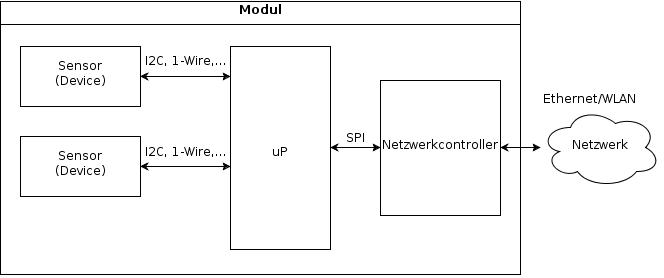
\includegraphics[width=0.5 \paperwidth]{./bilder/modul_aufbau.png}
	\caption{Aufbau eines Moduls}
	\label{modulaufbau}
	\end{center}
	\end{minipage}
}
\end{center}
\end{figure}

\newpage

Sie vereinen alle benötigten Komponenten - Mess- und Netzwerkeinheit - auf einer Platine (siehe Abb. \ref{modulaufbau}). Hier erfolgt die Übertragung zwischen den Sensoren und dem Mikroprozessor (uP) meist über Schnittstellen, wie I2C oder 1-Wire, während der Netzwerkcontroller per SPI mit dem uP kommuniziert. Über TCP und mit den beiden Protokollen \textit{netfind} und \textit{netcon} erfolgt die Abfrage und Steuerung durch den plattformunabhängigen Verwaltungs-Deamon \textit{netcond}. Näheres dazu im nächsten Abschnitt. 

\textbf{Messmodule} umfassen beispielsweise Sensoren für Temperatur, Luftdruck und Zeit. Jeder dieser Sensoren wird von netcon als \textbf{Device} bezeichnet und kann mit seiner ID abgefragt werden.

Um den Modulen automatisch eine IP-Adresse zuweisen zu können und damit Konfigurationsarbeit zu ersparen, sollten diese auch das DHCP-Protokoll unterstützen.

Es bestehen grundsätzlich drei Möglichkeiten zur Erstellung von Modulen. Wenn Sie alle erforderlichen Kenntnisse besitzen, um die gesamte Entwicklung selbst zu übernehmen, informieren Sie sich im Kapitel Hardware über den Aufbau der netcon-Protokolle. Sind Sie in der Lage einfache Messmodule ohne Netzwerkfähigkeit zu erstellen, verbinden Sie doch ein zusätzliches Netzwerkmodul (siehe Abb. \ref{modulaufbau2}). Diese Möglichkeit erfordert lediglich die Implementierung der Seriellen Schnittstelle (UART). Genauso können die im Rahmen dieser Diplomarbeit konzpierten Module mit ihrer Firmware für die Erstellung eigener Module herangezogen werden. Egal welche Wahl Sie treffen, das Kapitel Hardware unterstützt Sie in allen drei Fällen.

\begin{figure}[h]
\begin{center}
\fbox{
	%Rahmengroesse	
	\begin{minipage}{0.8 \paperwidth}
	\begin{center}
	%Bildgroesse
	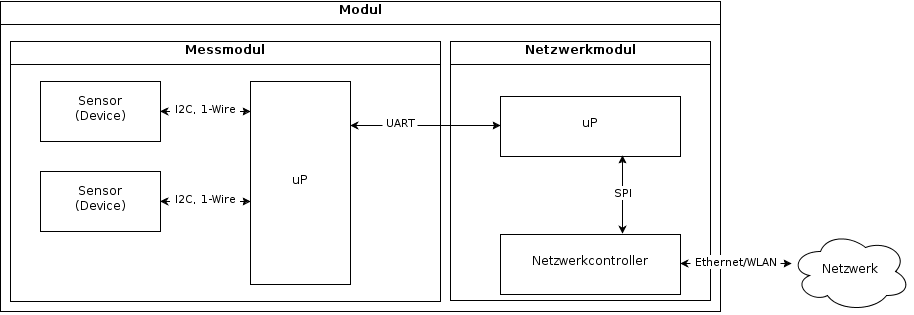
\includegraphics[width=0.7 \paperwidth]{./bilder/modul_aufbau2.png}
	\caption{Netzwerkfähiges Messmodul mittels LAN-UART Umsetzer}
	\label{modulaufbau2}
	\end{center}
	\end{minipage}
}
\end{center}
\end{figure}

\newpage

\subsubsection{Software}
Die Verwaltungsschnittstelle \textbf{netcond} ist eine in Java geschriebene Hintergrundanwendung (Daemon), die sich um die Verwaltung der Module kümmert. Wie in Abb. \ref{netcond} erkennbar können über das netcon Application Interface (netcon API) per TCP die Moduldaten abgefragt werden. Die Anwendung kann beispielsweise eine Website auf einem Webserver oder ein Smartphone-App sein. 

\begin{figure}[h]
\begin{center}
\fbox{
	%Rahmengroesse	
	\begin{minipage}{0.7 \paperwidth}
	\begin{center}
	%Bildgroesse
	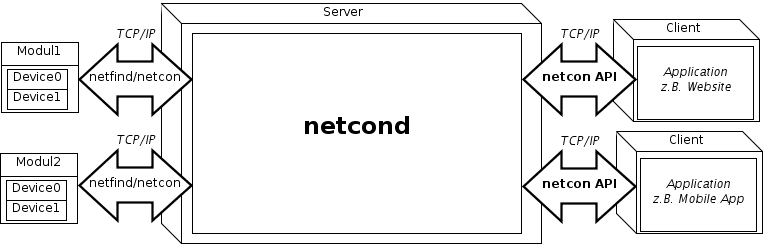
\includegraphics[width=0.7 \paperwidth]{./bilder/netcond.png}
	\caption{netcond}
	\label{netcond}
	\end{center}
	\end{minipage}
}
\end{center}
\end{figure}

\newpage
Soll die Anwendung zur Anzeige der Messdaten selbst entwickelt werden, führt das Kapitel Software in die Verwendung der Softwareschnittstelle ein. Sonst kann die bereits entwickelte Website \textbf{netcon web} (siehe Abb. \ref{website}) verwendet werden. Dazu ist zusätzlich zur JRE ein http-Webserver mit PHP-Unterstützung erforderlich. Deren Installation und Konfiguration ist im Kapitel Software erklärt. 

\begin{figure}[h]
\begin{center}
\fbox{
	%Rahmengroesse	
	\begin{minipage}{0.7 \paperwidth}
	\begin{center}
	%Bildgroesse
	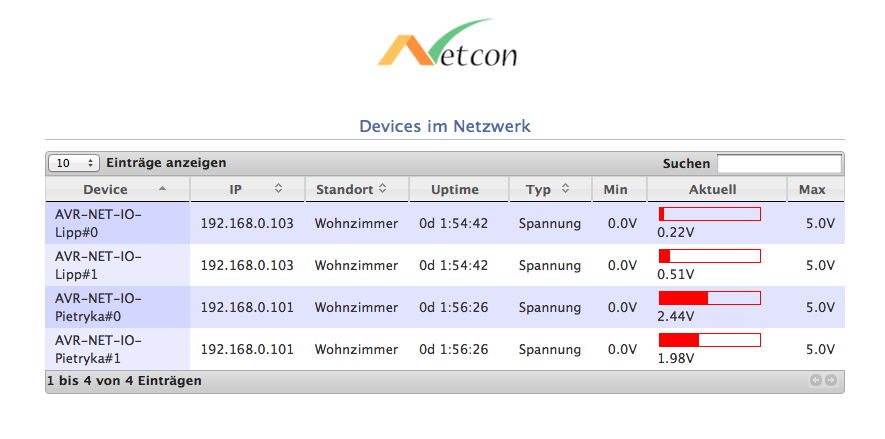
\includegraphics[width=0.7 \paperwidth]{./bilder/website.png}
	\caption{netcon web}
	\label{website}
	\end{center}
	\end{minipage}
}
\end{center}
\end{figure}

\newpage

\section{Grundlagen [Pietryka]}
\subsection{OSI-Schichtenmodell}
Das OSI-Schichtenmodell ist ein von der ISO im Jahre 1983 standardisiertes Modell, welches als Designgrundlage für Kommunikationsprotokolle in Computernetzen dient. Dabei wird die Kommunikation beim OSI-Modell auf sieben Schichten bzw. Layern aufgeteil. Für jede dieser Schichten sind Anforderungen und Aufgaben definiert, welche von entsprechenden Protokollen realisiert werden müssen. Eine konkrete Umsetzung ist aber nicht vorgegeben, daher gibt es für eine Schicht mehrere in Frage kommenden Protokolle.
\subsubsection{Schicht 1: Bitübertragungsschicht}
Protokolle auf dieser Schicht kümmern sich darum, wie die unterschiedlichen Netzwerkgeräte untereinander verbunden sind, sowie welches Medium dafür verwendet wird. Hier geht es um die Übertragung einzelner Bits, es müssen je nach Übertragungsmedium verschiedene Codes oder Modulationsverfahren für die Übertragung von einzelnen Bits Festgelegt werden. Weiterhin sind Geräte wie Antennen, Verstärker, Stecker und Buchsen ebenfalls auf dieser Schicht definiert.

Protokolle und Normen: V.24, V.28, X.21, RS 232, RS 422, RS 423, RS 499

\subsubsection{Schicht 2: Sicherungsschicht}
Auf dieser Schicht definierte Protokolle, sollen sich darum kümmern, dass die Daten zuverlässig, im Sinnen von fehlerfrei, ankommen. Dazu wird der Bitstrom in Blöcke (auch Frames genannt) unterteilt, diese Frames werden mit einer Prüfsumme versehen, welches es dem Empfänger erlaubt Fehler zu erkennen und ja nach Protokoll auch Fehler bis zu einem gewissen Grad zu korrigieren. Ein erneutes Anfordern von verworfenen Blöcken, oder das Erkennen von überhaupt nicht angekommenen Blöcken ist auf dieser Schicht nicht vorgesehen. Weiterhin findet wird im Protokoll eine sogenannte Zugriffskontrolle definiert, diese regelt, wann und wer auf das Medium zugreifen darf. Hardwareelemente auf dieser Schicht sind die Bridge und der Switch.

Bekannte Protokolle auf dieser Schicht sind das Ethernet-Protokoll, welches besser als das kabelgebundene lokale Netzwerk bekannt ist, oder das IEEE 802.11 Protokoll, welches das bekannte Wireless-LAN beschreibt.

\subsubsection{Schicht 3: Vermittlungsschicht}
Diese Schicht kümmert sich um das Weiterleiten von Paketen bei paketorientierten Diensten. Meist besteht zwischen Sender und Empfänger keine direkte Verbindung, daher muss das Paket mehrere Zwischenstationen durchlaufen bis es an seinem Ziel ankommt. Dieser Vorgang wird Routing genannt, die Hardware für diese Schicht ist der Router.

Protokolle und Normen: X.25, ISO 8208, ISO 8473 (CLNP), ISO 9542 (ESIS), IP, IPsec, ICMP

\subsubsection{Schicht 4: Transportschicht}
Die Aufgabe dieser Schicht ist einerseits die Stauvermeidung, andererseits Stellt diese Schicht mit ihren Protokollen für die höheren Schichten einen einheitlichen Zugriff. Deswegen müssen die höheren Schichten auch nicht wissen welche Protokolle auf den unteren Schichten arbeiten. Bekannte Protokolle sind TCP, welches bereits die Datensicherheit durch Neuübertragungen vorgesehen hat, sowie UDP, welches, außer einer Prüfsumme, keine Sicherheitsmechanismen hat.

\subsubsection{Schicht 5: Sitzungsschicht}
Die Sitzungsschicht sorgt für die Prozesskommunikation zwischen zwei Systemen, Sie sorgt dafür, dass Zusammenbrüche einer Sitzung oder Ähnliche Störungen behoben werden. Dazu werden sogenannte Wiederaufsetzpunkte eingeführt, an denen die Sitzung nach einem Ausfall der Verbindung wieder fortgesetzt werden kann.

\subsubsection{Schicht 6: Darstellungsschicht}
Bei der Darstellungsschicht geht es darum, die systemabhängige Darstellung der Daten in eine unabhängige Form zu bringen. Diese erlaubt den korrekten Datenaustausch zwischen zwei unterschiedlichen Systemen. Ebenfalls zur Schicht 6 gehören Verschlüsselung und Datenkompression, sowie eventuell das Übersetzen zwischen verschiedenen Datenformaten.

\subsubsection{Schicht 7: Anwendungsschicht}
Die oberste Schicht, die sogenannte Anwendunsschicht verschafft Anwendungen den Zugriff zum Netz. Hierzu zählen Alle Anwendungen die einem Netzwerkkommunikation Benötigen wie E-Mail Client, Browser, etc.

Protokolle auf dieser Schicht sind unter Anderem HTTP, FTP, SSH, Telnet, etc.
 
\subsection{Ethernet}


\subsubsection{MAC-Adresse}
Die MAC-Adresse (Media-Access-Controll-Adresse) ist eine Adresse welche Netzwerkgeräte eindeutig identifiziert, Ethernet Pakete werden mithilfe dieser Adresse adressiert. Diese Adresse ist 48-Bit lang und ist auf der Welt eindeutig für jedes Netzwerkgerät. Die Darstellung erfolgt in Hexadezimaler Darstellung wie 00:80:41:ae:fd:7e oder 00-80-41-ae-fd-7e. Will man seine Netzwerkfähigen Geräte am Markt verkaufen, so benötigt man gültige MAC-Adressen, diese kann man in Blöcken kaufen. Kleinere Unternehmen können Blöcke mit 4096 MAC-Adressen kaufen, größere Unternehmen besitzen die Möglichkeit einen Block mit 16,8 Millionen Adressen zu kaufen.

Entwickelt man aber noch geringere Stückzahlen, so gibt es beispielsweise von der Firma Microchip EEPROMS, welche mit einer bereits vorprogrammierten und natürlich gültigen MAC-Adresse geliefert werden. Eine weitere Möglichkeit gültige MAC-Adressen während der Entwicklung zu vergeben sind die sogenannten lokal administrierten Adressen, dabei wird im ersten Byte das zweite Bit auf 1 gesetzt. Ist dies der Fall, so handelt es sich um eine lokal administrierte Adresse, der Nachteil hierbei ist natürlich, dass diese Adresse nicht mehr eindeutig ist.

\subsubsection{Broadcast}
Bei einem sogenannten Broadcast wird im Ethernet-Header eine spezielle MAC-Adresse als Ziel angegeben, nämlich FF:FF:FF:FF:FF:FF, Pakete mit dieser Zieladresse werden an alle Geräte in einem LAN-Netzwerk verschickt, jedoch nicht in ein anderes Netzwerk geroutet.

\subsection{IP}

\subsection{ARP}

\subsection{TCP}

\subsection{UDP}

\subsection{DHCP}

\newpage

\section{Hardware [Pietryka]}
\subsection{Der Ethernet Controller}
\subsection{Auswahl des Ethernet Controllers}
Damit ein Mikrocontroller über das Ethernet kommunizieren kann, wird eine entsprechende Hardware benötigt, der sogenannte Ethernet Controller. Ein Ethernet Controller übernimmt dabei die Aufgaben der OSI-Schichten 1(Physical) und 2(Data-Link). Der Controller benötigt zudem einen entsprechend großen Empfangspuffer, um mindestens einen vollwertigen Ethernet-Frame(1542 Byte) aufzunehmen zu können. Dabei standen für 8-Bit Mikrocontroller vorerst zwei verschiedene Bausteine zur Auswahl, einmal der CP2200 von SiLabs, und einmal der ENC28J60 von Microchip. Beide Controller haben, was die Netzwerkkommunikation angeht, so ziemlich die selben Features, der gravierende Unterschied liegt jedoch in der Ansteuerung dieser. Der CP2200 wurde von SiLabs, wie es scheint, nur für die Verwendung mit einem Mikrocontroller vom Typ 8051 entwickelt, die Ansteuerung erfolgt deshalb über einen parallelen Adress-/Datenbus wodurch man mindestens 16 Leitungen und Pins am Mikrocontroller benötigt. Beim ENC28J60 erfolgt die Kommunikation über den SPI-Bus, daher benötigt man nur vier Leitungen(MOSI, MISO, SCK, CS), dadurch hat auch der Netzwerkcontroller selber nur 28 Pins und ist auch im "bastlerfreundlichen" DIP-Gehäuse zu bekommen. Ein anderer Faktor für die Auswahl des ENC28J60 war das Vorhandensein einer günstigen Entwicklungsplatine, es gibt bei Pollin den AVR-NET-IO Bausatz, dieser kostet nur \EUR{20} und enthält alle für die Netzwerkprogrammierung benötigten Komponenten(ATmega32, ENC28J60, RJ-45 Buchse).

\subsection{ENC28J60 Beschaltung}
Die Aussenbeschaltung benötigt neben einigen Standardbauelementen auch einige 1\% Widerstände und einen 1:1 Übertrager, jedoch gib es RJ-45 Buchsen in denen bereits der Übertrager, sowie die LEDs bereits eingebaut sind.
\begin{figure}[h]
\begin{center}
\fbox{
	%Rahmengroesse	
	\begin{minipage}{0.7 \paperwidth}
	\begin{center}
	%Bildgroesse
	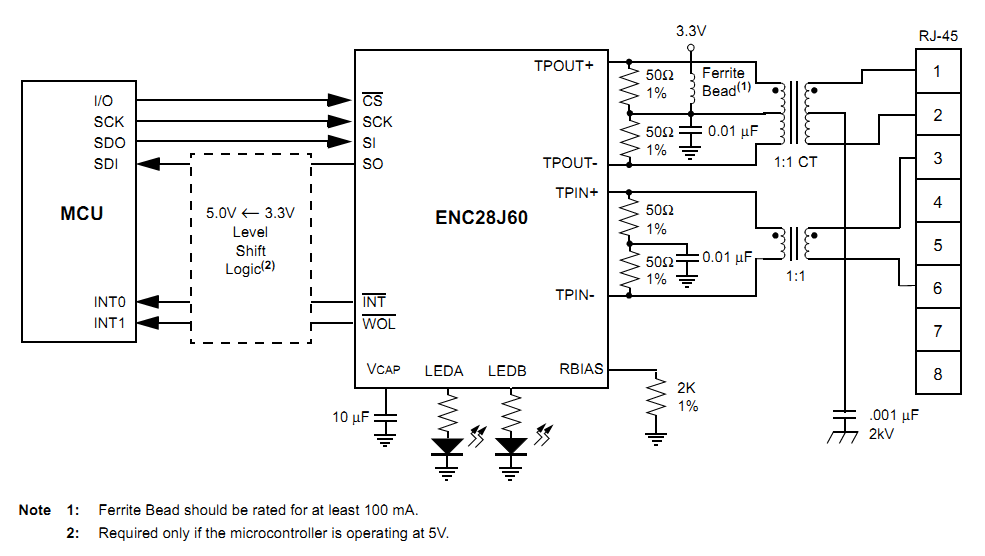
\includegraphics[width=0.7 \paperwidth]{./bilder/enc28j60_beschaltung.png}
	\caption{Aussenbeschaltung ENC28J60}
	\end{center}
	\end{minipage}
}
\end{center}
\end{figure}

\subsection{ENC28J60 Treibersoftware}
Die erste Aufgabe war es eine Bibliothek zu schreiben, welche es erlaubt, mithilfe des ENC28J60, Ethernet Pakete über das Netzwerk zu verschicken. Es waren zwar im Internet verschiedene Programme für den ENC28J60 vorhanden, diese waren aber teilweise schlampig und unschön geschrieben. Am Ende Stand eine Bibliothek zur Verfügung, die auch für andere Projekte genutzt werden kann, diese wurde für den AVR geschrieben und besteht aus zwei Dateien "enc28j60.h" und "enc28j60.c". Zurzeit übernimmt die Bibliothek auch die Initialisierung des SPI-Busses, will man dies verhindern, so muss man die Zeilen 187-197 in der Datei "enc28j60.c" entfernen, weiterhin wird es eventuell nötig sein die  Pins für das Chip-Select anzupassen, dazu muss man die Funktionen get\_cs() und release\_cs() in den Zeilen 24-32 ebenfalls anpassen. Für die Benutzung der Bibliothek stehen dann drei Funktionen zur Verfügung. Die Bibliothek selber finde sich im Ordner "netcon Module/Pollin AVR-NET-IO/enc28j60/".

Der Treiber selbst kann als stabil angesehen werden, es sind in den mehreren Monaten der Arbeit mit diesem keine Fehler aufgefallen, auch wurde das Geräte mehrere Stunden über die Nacht laufen gelassen, mit Erfolg.

\subsubsection{void enc28j60\_init(const uint8\_t *mac\_addr)}
Initialisiert die Hardware des ENC28J60 mit der angegebenen MAC-Adresse, diese muss als ein Zeiger auf ein Array mit 6 Byte übergeben werden. Zurzeit wird auch die SPI-Hardware eines ATmega32 ebenfalls initialisiert, ist dies nicht gewünscht, so muss der Code entsprechend abgeändert werden.

\begin{quote}
\begin{verbatim}
const uint8_t mac_addr[6] = {0x02, 0x00, 0x00, 0x00, 0x00, 0x01};
enc28j60_init(mac_addr);
\end{verbatim}
\end{quote}

\subsubsection{void enc28j60\_transmit(const uint8\_t *data, uint16\_t len)}
Sendet ein Ethernet-Paket in das Netzwerk, welches über einen Zeiger auf data referenziert wurde, mit der Länge len.
\begin{quote}
\begin{verbatim}
uint8_t buf[512];

strcpy(buf, "Das ist ein ungueltiges Paket");
enc28j60_transmit(buf, strlen(buf));
\end{verbatim}
\end{quote}

\subsubsection{uint16\_t enc28j60\_receive(uint8\_t *data, uint16\_t max\_len)}
Schaut ob ein Paket im Puffer des ENC28J60 angekommen ist, ist dies der Fall, so werden bis zu max\_len Bytes in den durch data referenzierten Bereich kopiert. Als Rückgabewert liefert die Funktion die Anzahl der erfolgreich gelesenen Byte. Ist kein neues Paket beim Aufruf der Funktion vorhanden, so ist der Rückgabewert 0.
\begin{quote}
\begin{verbatim}
uint8_t buf[512], len;

while(1 > 0)
{
    len = enc28j60_receive(buf, 512);
    if(len > 1)
    {
        // Neues Paket
    }
}
\end{verbatim}
\end{quote}

\subsubsection{Ethernet-DK Port}
Weiterhin, wurde eine Portierung des ENC28J60C Treibers auf das Ethernet-DK von SiLabs durchgeführt. Dies lässt sich mit dem freien C-Compiler SDCC compilieren, die entsprechenden Projektdateien sind im Ordner "netcon Module/Ethernet-DK/enc28j60". Damit dieses Projekt erfolgreich compiliert muss der SDCC Compiler entsprechen in der SiLabs IDE eingestellt konfiguriert werden, zudem muss sowohl dem Linker als auch dem Compiler der Parameter "--model-large" übergeben werden.

\subsection{CP2200}
Auch wenn der CP2200 Ethernet-Controller nicht weiter verwendet wurde, so wurde ebenfalls ein Treiber geschrieben, sowie der uIP Stack auf diesen portiert, diese Projektdateien finden sich im Ordner "netcon Module/Ethernet-DK/cp2200". Über die Stabilität kann keine Auskunft gegeben werden, jedoch hat die Netzwerkkommunikation über eine Stunde hinweg funktioniert. Auf eine weitere Dokumentation wird hier verzichtet, da der Treiber nur als Nebenprodukt verschiedener Experimente anzusehen ist.

\subsection{Der uIP TCP/IP Stack}
Die Kommunikation der Module soll im Netzwerk über TCP ablaufen, zum einen damit gewährleistet ist, dass die Daten auch ankommen, zum anderen damit die Module mit allen Betriebssystemen, Programmiersprachen und Netzwerkbibliotheken kompatibel sind, denn dies ist nur durch TCP oder UDP der Fall, diese Protokolle sind in jedem modernen Betriebssystem ein fester Bestandteil. Eine Software die sich nun um das IP, TCP und eventuell auch um das UDP Protokoll kümmert, nennt man einen TCP/IP Stack.

Der von uns verwendetet Ethernet-Controller liefert uns jedoch nur Ethernet-Frames, daher benötigt man einen in Software geschriebenen TCP/IP Stack, einen solchen zu schreiben wäre an sich schon eine eigene Diplomarbeit, hinzu kommt noch die Tatsache, dass RAM-Speicher und Rechengeschwindigkeit des Prozessors begrenzt sind, das ganze soll ja auf einem ATmega32 mit 2K RAM laufen.

\subsection{DHCP Implementierung}

\subsection{netcon Serial Protocol}
Wie bereits erwähnt war es eines der Ziele, ein Netzwerkmodul zu entwickeln, welches es erlaubt andere Messgeräte "`einfach"' in das Messsystem einzubinden. Dazu kommuniziert das Netzwerkmodul mit dem Messgerät über die serielle Schnittstelle nach einem bestimmten Protokoll, dem netcon Serial Protocol. Die Messgeräte verhalten sich dabei passiv und erhalten vom Netzwerkmodul verschiedene Anfragen, diese sollte innerhalb von 50ms entsprechend beantwortet werden. Jegliche Kommunikation läuft dabei über den standardmäßigen ASCII-Zeichensatz.

Kommandos:
\begin{quote}
\begin{verbatim}
Anfrage: n
Antwort: <Name>\n
Fragt den Namen des Messgerätes ab.

Anfrage: o
Antwort: <Standort>\n
Fragt den Standort des Messgerätes ab.

Anfrage: a
Antwort: <Anzahl>\n
Fragt die Anzahl der Sensoren, die mit dem Messgerät gemessen
werden können ab, wobei Anzahl eine Zahl von 00-FF sein kann.

Anfrage: w##
Antwort: <Wert>\n
Fragt den aktuellsten Messwert von dem Sensor mit der Nummer
## ab.

Anfrage: f##
Antwort: <Format>\n
Fragt das Format für den Wert von Sensor ## ab.
Dieses gibt an wie der Wert an das Netzwerkmodul übergeben
wird, folgende Formate sind vorgesehen:
    h - Hexadezimal
    i - Dezimal
    f - Fließkommazahl
    
Anfrage: t##
Antwort: <Typ>\n
Fragt den Typ für den Sensor ## ab, dies soll es ermöglichen,
bei der Ausgabe nach Temperatursensoren, Luftdrucksensoren,
etc. zu filtern. Der Typ ist eine Zahl von 00-FF, jedoch
wurden noch keine Typen definiert.

Anfrage: m##
Antwort: <Minimum>\n
Fragt das Minimum des Sensors ## ab.

Anfrage: x##
Antwort: <Maximum>\n
Fragt das Maximum des Sensors ## ab.
\end{verbatim}
\end{quote}

Beim Einschalten des Netzwerkmoduls werden zuerst der Name, der Ort und die Anzahl der Sensoren abgefragt, anschließend wird für jeden Sensor das Format, der Typ, der Min und der Max Wert abgefragt. Nach dieser Initialisierung werden alle 500ms die aktuellen Werte alles Sensoren nacheinander abgefragt. Eine Implementierung dieses Protokolls befindet sich im Ordner "netcon Module/Pollin AVR-NET-IO/netcon\_ser", diese wurde bis jetzt nicht einem dauerhaften Test unterzogen, es könnten Fehler enthalten sein.

\newpage
\section{Software [Lipp]}

Das Kapitel beschreibt das Softwareinterface zwischen den Modulen und den Applikationen zur Anzeige der Moduldaten, um eigene Anwendungen, wie Webseiten oder Smartphone-Apps zu realisieren. Als Anwendungsbeispiel wurde bereits eine Website implementiert, die für den eigenen Gebrauch herangezogen werden kann.

\subsection{Aufgaben}
Die Software, genauer gesagt \textbf{netcond}, ist ein sogenannter Daemon (Hintergrundprozess), der im Allgemeinen die Module im Netzwerk verwaltet, indem er ihre Messwerte aufzeichnet, die über ein spezielles Interface abgefragt werden können. Auch modulseitig kommt ein eigens entwickeltes Protokoll zum Einsatz, das bereits im vorangegangenen Kapitel erklärt wurde. Wenn sich alle Module nach dieser Spezifikation verhalten, werden sie auch von netcond als solche erkannt.

\subsection{Java}

Die Anwendung wurde in Java geschrieben, um Plattformunabhängigkeit zu gewährleisten. Damit ist der Einsatz auf jeder Plattform möglich, die eine Java Runtime Environment (JRE) in Version 6 oder höher zur Verfügung stellt, egal ob PC, Server oder Embedded System. Die Installation dieser Laufzeitumgebung ist im Abschnitt Installation genau beschrieben. 

\newpage

\subsection{Hardwareanforderungen}
Netcond wurde für hardwareschwache Computer konzipiert. Demnach steht dem Einsatz auf eingebetteten Systemen nichts im Wege, Voraussetzung ist ausschließlich, wie bereits erwähnt, die Verfügbarkeit der JRE. 

Da der Daemon im Hintergrund läuft, muss das Betriebssystem über keine grafische Oberfläche verfügen. Netcond kann auf einem Server/Embedded System ohne Monitor über zum Beispiel SSH ausgeführt und gewartet werden. 

\textbf{Empfohlende Hardware}

\begin{itemize}
	\item 1 GHz CPU
	\item 64 MB RAM (nur für netcond)
	\item Netzwerkkarte
	\item Textbasiertes Betriebssystem mit SSH-Zugang
\end{itemize}

Soll eine eigene Website oder die dieser Diplomarbeit für die Anzeige der Moduldaten genutzt werden, ist weiters ein PHP-fähiger Webserver, wie zum Beispiel Apache erforderlich. Wenn dieser auf der selben Hardware laufen soll, wird zusätzlich Arbeitsspeicher benötigt. Die Installation eines Webservers wird im Abschnitt Installation für die gängigen Betriebssysteme beschrieben. 

\newpage

\subsection{Aufbau und Funktionsweise}

Der Java-Daemon netcond sucht nach dem Start alle paar Sekunden das Netzwerk nach verbunden Modulen ab und halt diese in einer Liste. Für jedes dieser Module wird ein neuer Programmfaden erzeugt, der ständig Messdaten abfragt und diese speichert. Zusätzlich startet der Daemon einen weiteren Subprozess, die Schnittstelle, über die eine Anwendung - in diesem Fall ein Webserver - die Daten abfragen kann. Verbindet sich ein Webbrowser zu diesem Webserver, weißt ein PHP-Script den Daemon an, die aktuellen Daten zu übermitteln. Diese werden dann auf der Website angezeigt. Dieses Prinzip ist nocheinmal in Abb. \ref{funktionsweise} grafisch verdeutlicht.

\begin{figure}[h]
\begin{center}
\fbox{
	%Rahmengroesse	
	\begin{minipage}{0.8 \paperwidth}
	\begin{center}
	%Bildgroesse
	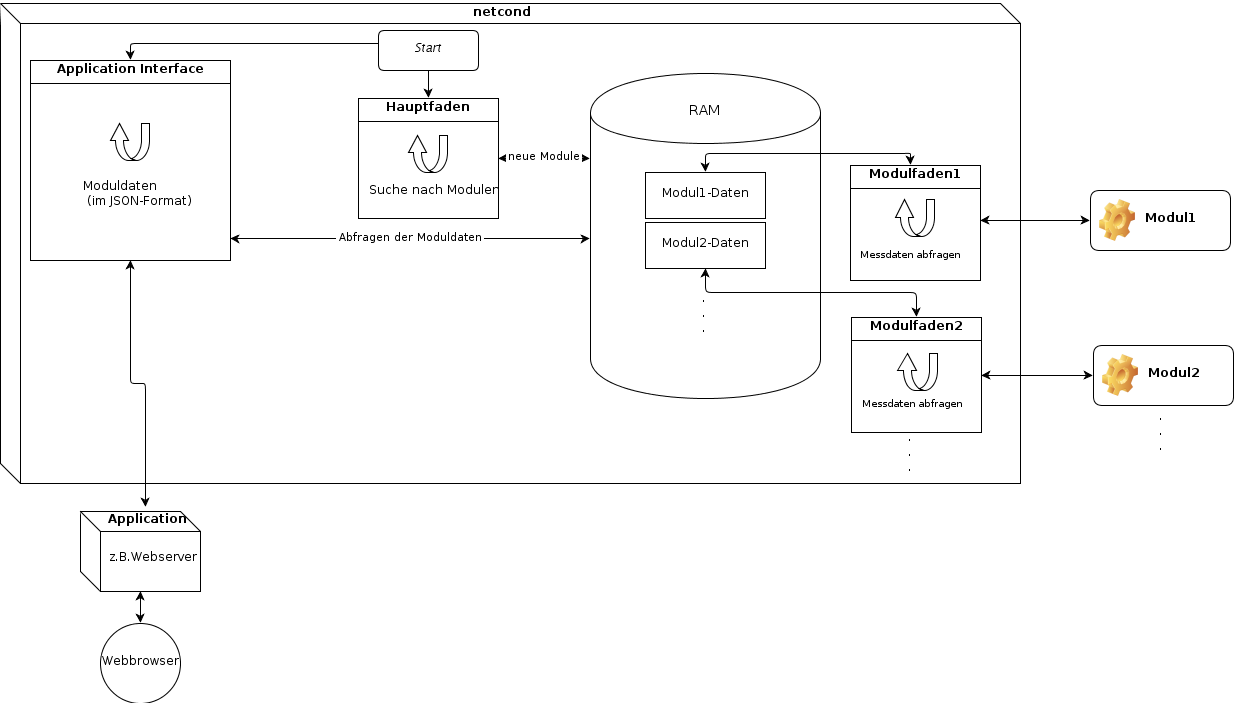
\includegraphics[width=0.8 \paperwidth]{./bilder/funktionsweise.png}
	\caption{netcon - Funktionsprinzip}
	\label{funktionsweise}
	\end{center}
	\end{minipage}
}
\end{center}
\end{figure}

\newpage

\subsection{Installation}

\subsubsection{JRE}

\subsubsection{Webserver}

 
\end{document}